\documentclass[]{article}
\usepackage{lmodern}
\usepackage{amssymb,amsmath}
\usepackage{ifxetex,ifluatex}
\usepackage{fixltx2e} % provides \textsubscript
\ifnum 0\ifxetex 1\fi\ifluatex 1\fi=0 % if pdftex
  \usepackage[T1]{fontenc}
  \usepackage[utf8]{inputenc}
\else % if luatex or xelatex
  \ifxetex
    \usepackage{mathspec}
  \else
    \usepackage{fontspec}
  \fi
  \defaultfontfeatures{Ligatures=TeX,Scale=MatchLowercase}
\fi
% use upquote if available, for straight quotes in verbatim environments
\IfFileExists{upquote.sty}{\usepackage{upquote}}{}
% use microtype if available
\IfFileExists{microtype.sty}{%
\usepackage{microtype}
\UseMicrotypeSet[protrusion]{basicmath} % disable protrusion for tt fonts
}{}
\usepackage[margin=1in]{geometry}
\usepackage{hyperref}
\hypersetup{unicode=true,
            pdftitle={Make your own conserv-o-gram},
            pdfborder={0 0 0},
            breaklinks=true}
\urlstyle{same}  % don't use monospace font for urls
\usepackage{color}
\usepackage{fancyvrb}
\newcommand{\VerbBar}{|}
\newcommand{\VERB}{\Verb[commandchars=\\\{\}]}
\DefineVerbatimEnvironment{Highlighting}{Verbatim}{commandchars=\\\{\}}
% Add ',fontsize=\small' for more characters per line
\usepackage{framed}
\definecolor{shadecolor}{RGB}{248,248,248}
\newenvironment{Shaded}{\begin{snugshade}}{\end{snugshade}}
\newcommand{\KeywordTok}[1]{\textcolor[rgb]{0.13,0.29,0.53}{\textbf{#1}}}
\newcommand{\DataTypeTok}[1]{\textcolor[rgb]{0.13,0.29,0.53}{#1}}
\newcommand{\DecValTok}[1]{\textcolor[rgb]{0.00,0.00,0.81}{#1}}
\newcommand{\BaseNTok}[1]{\textcolor[rgb]{0.00,0.00,0.81}{#1}}
\newcommand{\FloatTok}[1]{\textcolor[rgb]{0.00,0.00,0.81}{#1}}
\newcommand{\ConstantTok}[1]{\textcolor[rgb]{0.00,0.00,0.00}{#1}}
\newcommand{\CharTok}[1]{\textcolor[rgb]{0.31,0.60,0.02}{#1}}
\newcommand{\SpecialCharTok}[1]{\textcolor[rgb]{0.00,0.00,0.00}{#1}}
\newcommand{\StringTok}[1]{\textcolor[rgb]{0.31,0.60,0.02}{#1}}
\newcommand{\VerbatimStringTok}[1]{\textcolor[rgb]{0.31,0.60,0.02}{#1}}
\newcommand{\SpecialStringTok}[1]{\textcolor[rgb]{0.31,0.60,0.02}{#1}}
\newcommand{\ImportTok}[1]{#1}
\newcommand{\CommentTok}[1]{\textcolor[rgb]{0.56,0.35,0.01}{\textit{#1}}}
\newcommand{\DocumentationTok}[1]{\textcolor[rgb]{0.56,0.35,0.01}{\textbf{\textit{#1}}}}
\newcommand{\AnnotationTok}[1]{\textcolor[rgb]{0.56,0.35,0.01}{\textbf{\textit{#1}}}}
\newcommand{\CommentVarTok}[1]{\textcolor[rgb]{0.56,0.35,0.01}{\textbf{\textit{#1}}}}
\newcommand{\OtherTok}[1]{\textcolor[rgb]{0.56,0.35,0.01}{#1}}
\newcommand{\FunctionTok}[1]{\textcolor[rgb]{0.00,0.00,0.00}{#1}}
\newcommand{\VariableTok}[1]{\textcolor[rgb]{0.00,0.00,0.00}{#1}}
\newcommand{\ControlFlowTok}[1]{\textcolor[rgb]{0.13,0.29,0.53}{\textbf{#1}}}
\newcommand{\OperatorTok}[1]{\textcolor[rgb]{0.81,0.36,0.00}{\textbf{#1}}}
\newcommand{\BuiltInTok}[1]{#1}
\newcommand{\ExtensionTok}[1]{#1}
\newcommand{\PreprocessorTok}[1]{\textcolor[rgb]{0.56,0.35,0.01}{\textit{#1}}}
\newcommand{\AttributeTok}[1]{\textcolor[rgb]{0.77,0.63,0.00}{#1}}
\newcommand{\RegionMarkerTok}[1]{#1}
\newcommand{\InformationTok}[1]{\textcolor[rgb]{0.56,0.35,0.01}{\textbf{\textit{#1}}}}
\newcommand{\WarningTok}[1]{\textcolor[rgb]{0.56,0.35,0.01}{\textbf{\textit{#1}}}}
\newcommand{\AlertTok}[1]{\textcolor[rgb]{0.94,0.16,0.16}{#1}}
\newcommand{\ErrorTok}[1]{\textcolor[rgb]{0.64,0.00,0.00}{\textbf{#1}}}
\newcommand{\NormalTok}[1]{#1}
\usepackage{graphicx,grffile}
\makeatletter
\def\maxwidth{\ifdim\Gin@nat@width>\linewidth\linewidth\else\Gin@nat@width\fi}
\def\maxheight{\ifdim\Gin@nat@height>\textheight\textheight\else\Gin@nat@height\fi}
\makeatother
% Scale images if necessary, so that they will not overflow the page
% margins by default, and it is still possible to overwrite the defaults
% using explicit options in \includegraphics[width, height, ...]{}
\setkeys{Gin}{width=\maxwidth,height=\maxheight,keepaspectratio}
\IfFileExists{parskip.sty}{%
\usepackage{parskip}
}{% else
\setlength{\parindent}{0pt}
\setlength{\parskip}{6pt plus 2pt minus 1pt}
}
\setlength{\emergencystretch}{3em}  % prevent overfull lines
\providecommand{\tightlist}{%
  \setlength{\itemsep}{0pt}\setlength{\parskip}{0pt}}
\setcounter{secnumdepth}{0}
% Redefines (sub)paragraphs to behave more like sections
\ifx\paragraph\undefined\else
\let\oldparagraph\paragraph
\renewcommand{\paragraph}[1]{\oldparagraph{#1}\mbox{}}
\fi
\ifx\subparagraph\undefined\else
\let\oldsubparagraph\subparagraph
\renewcommand{\subparagraph}[1]{\oldsubparagraph{#1}\mbox{}}
\fi

%%% Use protect on footnotes to avoid problems with footnotes in titles
\let\rmarkdownfootnote\footnote%
\def\footnote{\protect\rmarkdownfootnote}

%%% Change title format to be more compact
\usepackage{titling}

% Create subtitle command for use in maketitle
\newcommand{\subtitle}[1]{
  \posttitle{
    \begin{center}\large#1\end{center}
    }
}

\setlength{\droptitle}{-2em}

  \title{Make your own `conserv-o-gram'}
    \pretitle{\vspace{\droptitle}\centering\huge}
  \posttitle{\par}
    \author{}
    \preauthor{}\postauthor{}
    \date{}
    \predate{}\postdate{}
  

\begin{document}
\maketitle

\section{Purpose}\label{purpose}

To summarize and visualize temporal changes in population trends for
species of conservation concern.

\begin{figure}
\centering
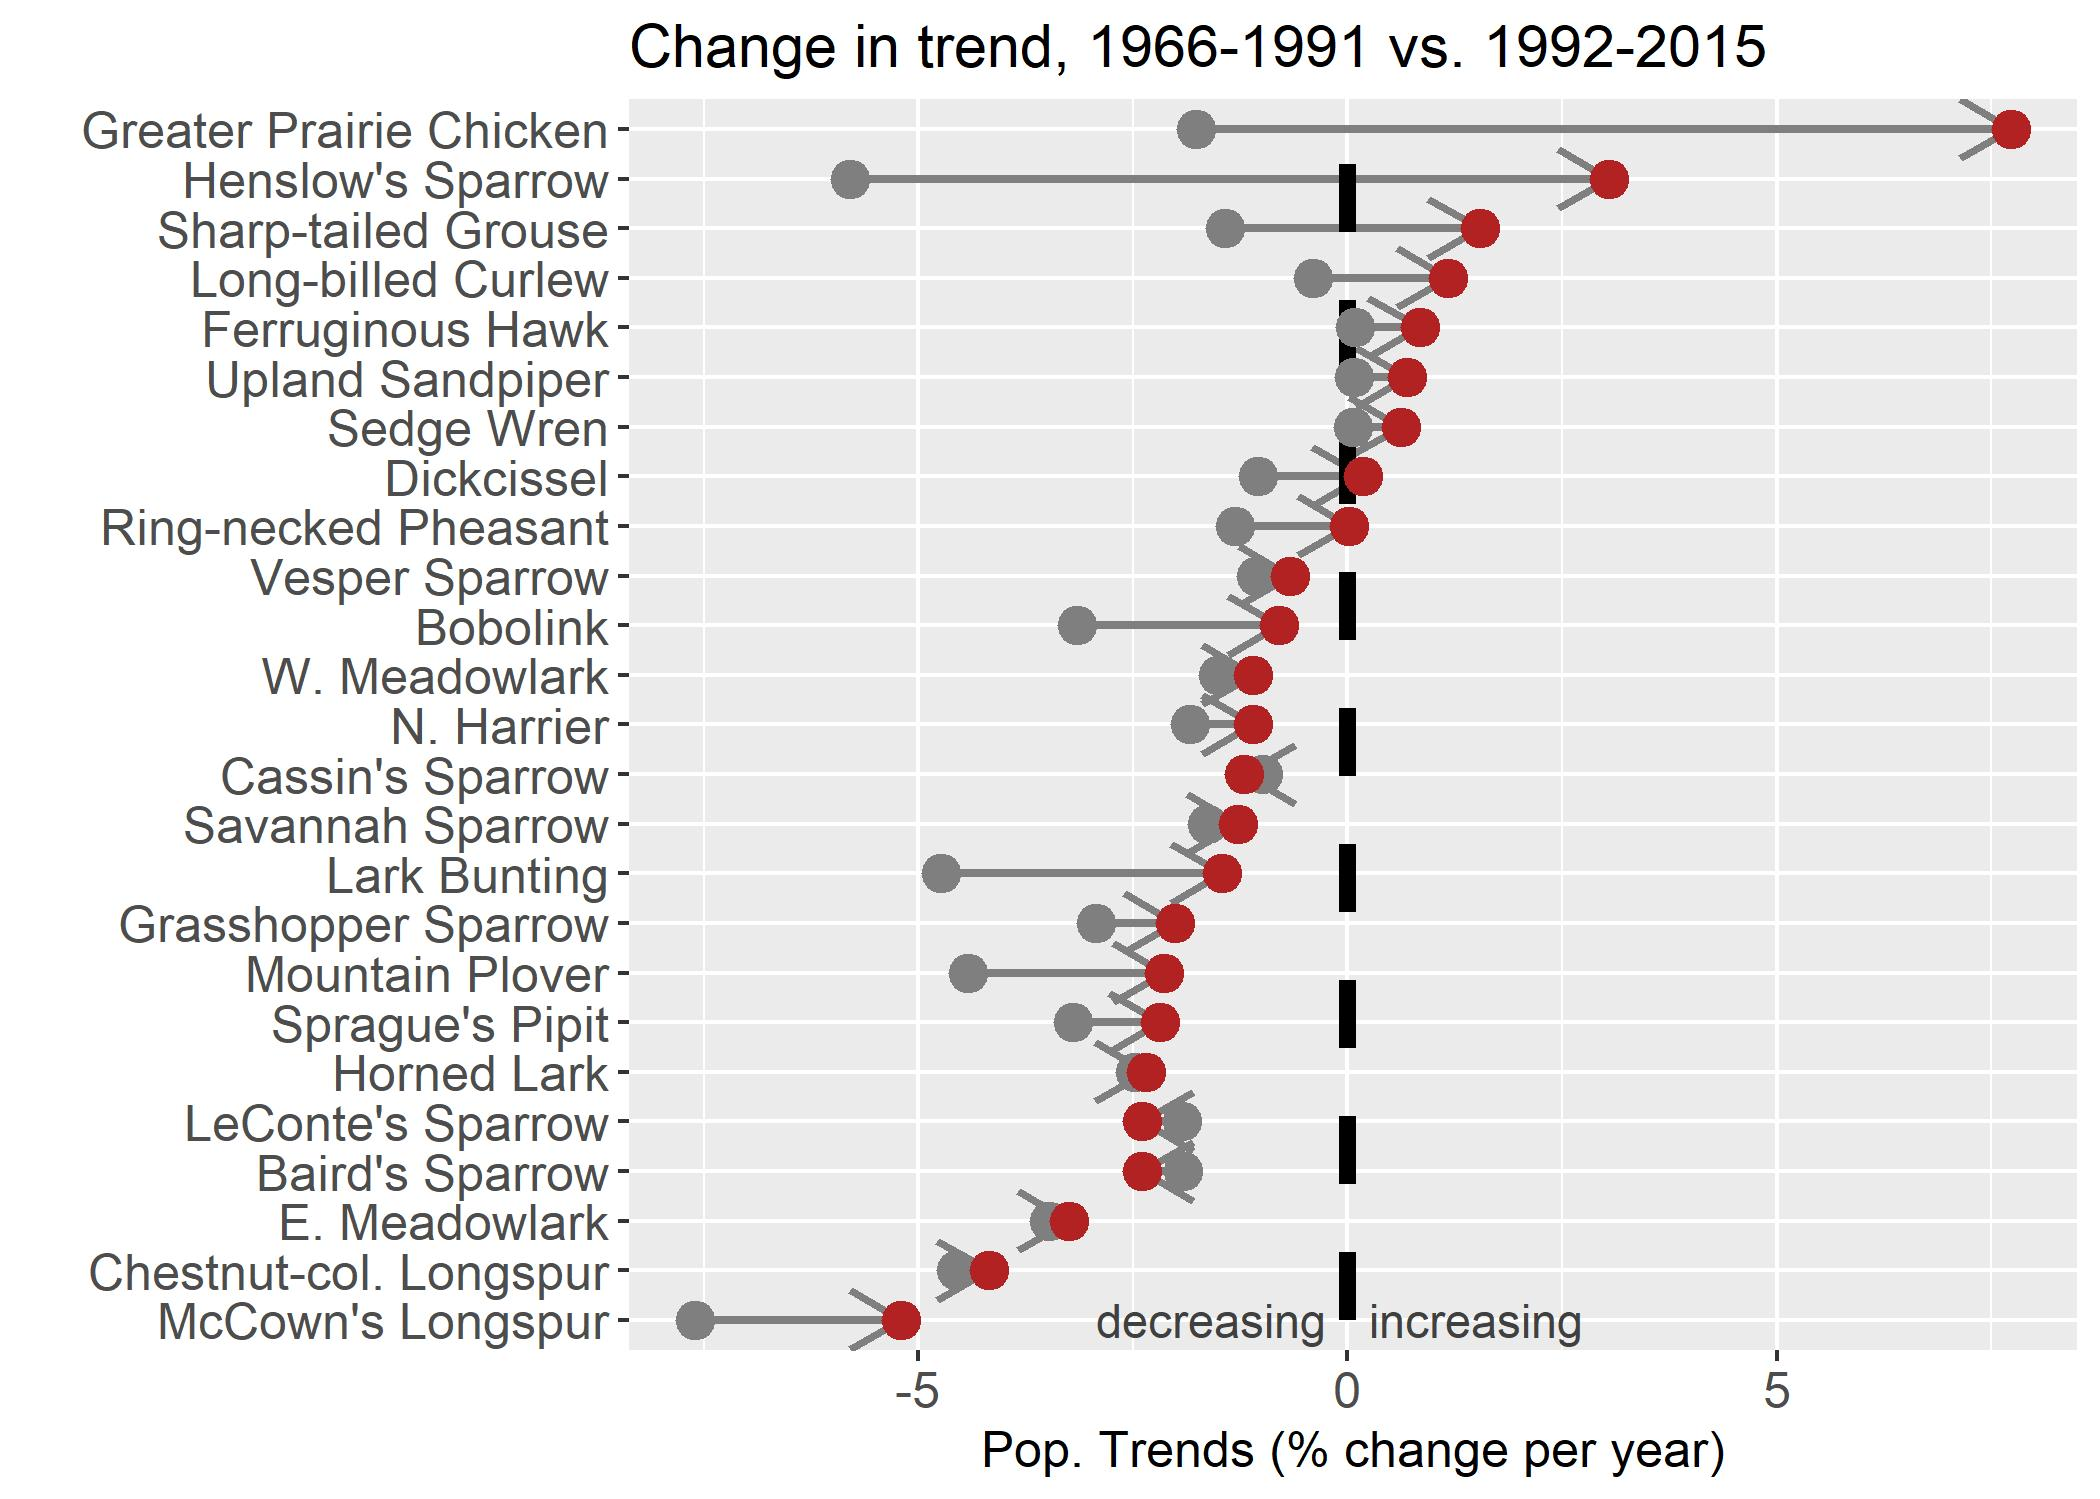
\includegraphics{C:/Users/Mike/Documents/Research/Conservation_dataviz/scripts/conservogram_grassland_birds.jpg}
\caption{Figure 1. A conservogram for grassland birds.}
\end{figure}

\section{Demo: Grassland birds in North
America}\label{demo-grassland-birds-in-north-america}

Trend info from \# \url{https://www.mbr-pwrc.usgs.gov/cgi-bin/tf15.pl}
(note: link not working at the moment!). This website provides custom
estimates of population trends for a given time period based on a
Bayesian hierarchical model of Breeding Bird Survey data.

\section{Load the required libraries}\label{load-the-required-libraries}

If needed, install them first using, for example:
install.packages(``ggplot2'')

\begin{Shaded}
\begin{Highlighting}[]
\KeywordTok{library}\NormalTok{(ggplot2)}
\KeywordTok{library}\NormalTok{(dplyr)}
\end{Highlighting}
\end{Shaded}

\begin{verbatim}
## 
## Attaching package: 'dplyr'
\end{verbatim}

\begin{verbatim}
## The following objects are masked from 'package:stats':
## 
##     filter, lag
\end{verbatim}

\begin{verbatim}
## The following objects are masked from 'package:base':
## 
##     intersect, setdiff, setequal, union
\end{verbatim}

\begin{Shaded}
\begin{Highlighting}[]
\KeywordTok{library}\NormalTok{(forcats)}
\end{Highlighting}
\end{Shaded}

\begin{verbatim}
## Warning: package 'forcats' was built under R version 3.5.3
\end{verbatim}

\section{Input the data}\label{input-the-data}

Note: in this case `historical' = 1966-1991, and `recent' = 1992-2015.
Customize with your own trend data from `historical' and `recent'
periods of your choice.

\begin{Shaded}
\begin{Highlighting}[]
\NormalTok{conservogram =}
\StringTok{  }\KeywordTok{tibble}\NormalTok{(}
    \DataTypeTok{species =} \KeywordTok{c}\NormalTok{(}
      \StringTok{"Long-billed Curlew"}\NormalTok{,}
      \StringTok{"Cassin's Sparrow"}\NormalTok{,}
      \StringTok{"Sedge Wren"}\NormalTok{,}
      \StringTok{"Baird's Sparrow"}\NormalTok{,}
      \StringTok{"Lark Bunting"}\NormalTok{,}
      \StringTok{"Dickcissel"}\NormalTok{,}
      \StringTok{"W. Meadowlark"}\NormalTok{,}
      \StringTok{"LeConte's Sparrow"}\NormalTok{,}
      \StringTok{"Savannah Sparrow"}\NormalTok{,}
      \StringTok{"Horned Lark"}\NormalTok{,}
      \StringTok{"Bobolink"}\NormalTok{,}
      \StringTok{"Upland Sandpiper"}\NormalTok{,}
      \StringTok{"Ring-necked Pheasant"}\NormalTok{,}
      \StringTok{"Chestnut-col. Longspur"}\NormalTok{,}
      \StringTok{"Grasshopper Sparrow"}\NormalTok{,}
      \StringTok{"Vesper Sparrow"}\NormalTok{,}
      \StringTok{"N. Harrier"}\NormalTok{,}
      \StringTok{"E. Meadowlark"}\NormalTok{,}
      \StringTok{"Sprague's Pipit"}\NormalTok{,}
      \StringTok{"McCown's Longspur"}\NormalTok{,}
      \StringTok{"Henslow's Sparrow"}\NormalTok{,}
      \StringTok{"Mountain Plover"}\NormalTok{,}
      \StringTok{"Greater Prairie Chicken"}\NormalTok{,}
      \StringTok{"Sharp-tailed Grouse"}\NormalTok{,}
      \StringTok{"Ferruginous Hawk"}
\NormalTok{    ),}
  
\DataTypeTok{trend.historical =} \KeywordTok{c}\NormalTok{(}\OperatorTok{-}\FloatTok{0.40}\NormalTok{,}\OperatorTok{-}\FloatTok{0.98}\NormalTok{,}\FloatTok{0.07}\NormalTok{,}\OperatorTok{-}\FloatTok{1.92}\NormalTok{,}\OperatorTok{-}\FloatTok{4.74}\NormalTok{,}\OperatorTok{-}\FloatTok{1.04}\NormalTok{,}\OperatorTok{-}\FloatTok{1.51}\NormalTok{,}\OperatorTok{-}\FloatTok{1.93}\NormalTok{,}\OperatorTok{-}\FloatTok{1.63}\NormalTok{,}\OperatorTok{-}\FloatTok{2.47}\NormalTok{,}\OperatorTok{-}\FloatTok{3.15}\NormalTok{,}\FloatTok{0.08}\NormalTok{,}
                         \OperatorTok{-}\FloatTok{1.31}\NormalTok{,}\OperatorTok{-}\FloatTok{4.56}\NormalTok{,}\OperatorTok{-}\FloatTok{2.93}\NormalTok{,}\OperatorTok{-}\FloatTok{1.06}\NormalTok{,}\OperatorTok{-}\FloatTok{1.83}\NormalTok{,}\OperatorTok{-}\FloatTok{3.48}\NormalTok{,}\OperatorTok{-}\FloatTok{3.20}\NormalTok{,}\OperatorTok{-}\FloatTok{7.6}\NormalTok{,}\OperatorTok{-}\FloatTok{5.8}\NormalTok{,}\OperatorTok{-}\FloatTok{4.42}\NormalTok{,}\OperatorTok{-}\FloatTok{1.76}\NormalTok{,}\OperatorTok{-}\FloatTok{1.43}\NormalTok{,}\FloatTok{0.09}\NormalTok{),}
\DataTypeTok{trend.recent =} \KeywordTok{c}\NormalTok{(}\FloatTok{1.17}\NormalTok{,}\OperatorTok{-}\FloatTok{1.21}\NormalTok{,}\FloatTok{0.62}\NormalTok{,}\OperatorTok{-}\FloatTok{2.39}\NormalTok{,}\OperatorTok{-}\FloatTok{1.46}\NormalTok{,}\FloatTok{0.18}\NormalTok{,}\OperatorTok{-}\FloatTok{1.10}\NormalTok{,}\OperatorTok{-}\FloatTok{2.39}\NormalTok{,}\OperatorTok{-}\FloatTok{1.27}\NormalTok{,}\OperatorTok{-}\FloatTok{2.35}\NormalTok{,}\OperatorTok{-}\FloatTok{0.80}\NormalTok{,}\FloatTok{0.70}\NormalTok{,}\FloatTok{0.02}\NormalTok{,}
                         \OperatorTok{-}\FloatTok{4.18}\NormalTok{,}\OperatorTok{-}\FloatTok{2.01}\NormalTok{,}\OperatorTok{-}\FloatTok{0.67}\NormalTok{,}\OperatorTok{-}\FloatTok{1.10}\NormalTok{,}\OperatorTok{-}\FloatTok{3.24}\NormalTok{,}\OperatorTok{-}\FloatTok{2.18}\NormalTok{,}\OperatorTok{-}\FloatTok{5.2}\NormalTok{,}\FloatTok{3.05}\NormalTok{,}\OperatorTok{-}\FloatTok{2.14}\NormalTok{,}\FloatTok{7.73}\NormalTok{,}\FloatTok{1.54}\NormalTok{,}\FloatTok{0.84}\NormalTok{)}
\NormalTok{)}
\end{Highlighting}
\end{Shaded}

\section{Make the graph}\label{make-the-graph}

\begin{Shaded}
\begin{Highlighting}[]
\KeywordTok{x11}\NormalTok{(}\DecValTok{7}\NormalTok{,}\DecValTok{7}\NormalTok{) }\CommentTok{# this makes a custom plot area 'pop out' if desired (inches x inches)}
\NormalTok{conservogram }\OperatorTok
\StringTok{  }\KeywordTok{mutate}\NormalTok{(}\DataTypeTok{species =} \KeywordTok{fct_reorder}\NormalTok{(species, trend.recent)) }\OperatorTok
\StringTok{  }\KeywordTok{ggplot}\NormalTok{() }\OperatorTok{+}
\StringTok{  }\KeywordTok{geom_segment}\NormalTok{(}\KeywordTok{aes}\NormalTok{(}\DataTypeTok{x =}\NormalTok{ trend.historical, }\DataTypeTok{y =}\NormalTok{ species, }\DataTypeTok{xend =}\NormalTok{ trend.recent, }\DataTypeTok{yend =}\NormalTok{ species), }\DataTypeTok{size =} \DecValTok{1}\NormalTok{, }
               \DataTypeTok{color =} \StringTok{"gray50"}\NormalTok{, }\DataTypeTok{arrow =} \KeywordTok{arrow}\NormalTok{(}\DataTypeTok{length =} \KeywordTok{unit}\NormalTok{(.}\DecValTok{5}\NormalTok{,}\StringTok{"cm"}\NormalTok{))) }\OperatorTok{+}
\StringTok{  }\KeywordTok{geom_segment}\NormalTok{(}\KeywordTok{aes}\NormalTok{(}\DataTypeTok{x =} \DecValTok{0}\NormalTok{, }\DataTypeTok{y =} \DecValTok{1}\NormalTok{, }\DataTypeTok{xend =} \DecValTok{0}\NormalTok{, }\DataTypeTok{yend =} \DecValTok{25}\NormalTok{), }\DataTypeTok{size =} \DecValTok{2}\NormalTok{, }\DataTypeTok{color =} \StringTok{"black"}\NormalTok{, }\DataTypeTok{linetype =} \DecValTok{2}\NormalTok{) }\OperatorTok{+}
\StringTok{  }\KeywordTok{geom_point}\NormalTok{(}\KeywordTok{aes}\NormalTok{(}\DataTypeTok{x=}\NormalTok{trend.historical, }\DataTypeTok{y =}\NormalTok{ species), }\DataTypeTok{size =} \DecValTok{4}\NormalTok{, }\DataTypeTok{color =} \StringTok{"gray50"}\NormalTok{) }\OperatorTok{+}
\StringTok{  }\KeywordTok{geom_point}\NormalTok{(}\KeywordTok{aes}\NormalTok{(}\DataTypeTok{x=}\NormalTok{trend.recent, }\DataTypeTok{y =}\NormalTok{ species), }\DataTypeTok{size =} \DecValTok{4}\NormalTok{, }\DataTypeTok{color =} \StringTok{"firebrick"}\NormalTok{) }\OperatorTok{+}
\StringTok{  }\KeywordTok{labs}\NormalTok{(}\DataTypeTok{x =} \StringTok{"Pop. Trends (% change per year)"}\NormalTok{, }\DataTypeTok{y =} \StringTok{""}\NormalTok{) }\OperatorTok{+}
\StringTok{  }\KeywordTok{labs}\NormalTok{(}\DataTypeTok{title =} \StringTok{"Change in trend, 1966-1991 vs. 1992-2015"}\NormalTok{) }\OperatorTok{+}
\StringTok{  }\KeywordTok{theme}\NormalTok{(}\DataTypeTok{axis.text =} \KeywordTok{element_text}\NormalTok{(}\DataTypeTok{size =} \DecValTok{12}\NormalTok{), }\DataTypeTok{title =} \KeywordTok{element_text}\NormalTok{(}\DataTypeTok{size =} \DecValTok{12}\NormalTok{)) }\OperatorTok{+}
\StringTok{  }\KeywordTok{annotate}\NormalTok{(}\StringTok{"text"}\NormalTok{, }\DataTypeTok{x =} \KeywordTok{c}\NormalTok{(}\OperatorTok{-}\NormalTok{.}\DecValTok{25}\NormalTok{, .}\DecValTok{25}\NormalTok{), }\DataTypeTok{y =} \DecValTok{1}\NormalTok{, }
           \DataTypeTok{label =} \KeywordTok{c}\NormalTok{(}\StringTok{"decreasing"}\NormalTok{,}\StringTok{"increasing"}\NormalTok{),}
           \DataTypeTok{hjust =} \KeywordTok{c}\NormalTok{(}\DecValTok{1}\NormalTok{,}\DecValTok{0}\NormalTok{), }\DataTypeTok{color =} \StringTok{"gray25"}\NormalTok{, }\DataTypeTok{size=}\DecValTok{4}\NormalTok{)}
\end{Highlighting}
\end{Shaded}

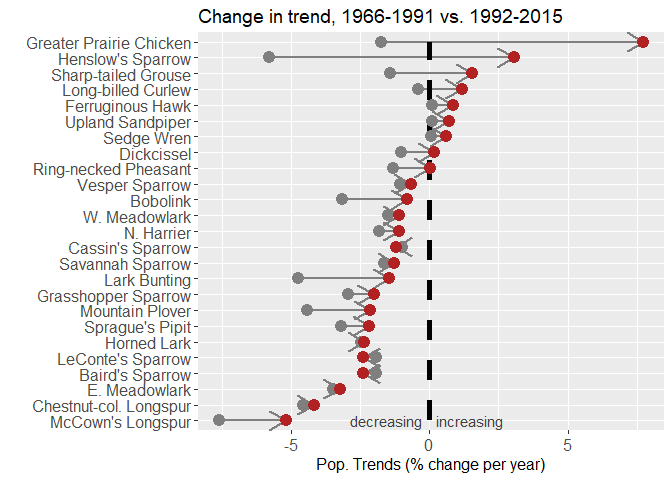
\includegraphics{Conservogram_files/figure-latex/unnamed-chunk-3-1.pdf}

\section{Save the graph}\label{save-the-graph}

You can save the last graph you made to a jpg or various other formats
(just change the extension) using the following command. It will save to
your working directory which you can view using: getwd()

\begin{Shaded}
\begin{Highlighting}[]
\KeywordTok{ggsave}\NormalTok{(}\StringTok{"conservogram_grassland_birds.jpg"}\NormalTok{)}
\end{Highlighting}
\end{Shaded}

\begin{verbatim}
## Saving 6.5 x 4.5 in image
\end{verbatim}


\end{document}
